\documentclass{beamer}
\usepackage[ngerman]{babel}
\usepackage[utf8]{inputenc}
\usepackage{graphicx}
\usepackage{amsmath}
\usepackage{amssymb}
\usepackage{dsfont}
\usepackage[T1]{fontenc}
\usepackage{pstricks}
\usepackage{pst-node}
%\usepackage[english]{babel}
%\usepackage[fixlanguage]{babelbib}
\usepackage{multimedia}


\usetheme{Warsaw}
%\useinnertheme{rounded}
\useoutertheme{infolines}

\title[Einführung in DEC]{Einführung in das Kalkül diskreter Differentialformen (DEC)}
\author{Ingo Nitschke}
\institute{IWR - TU Dresden}

\beamertemplatenavigationsymbolsempty

\newcommand{\R}{\mathds{R}}
\newcommand{\eps}{\varepsilon}
\newcommand{\qqquad}{\qquad\qquad}
\newcommand{\rot}{\text{rot}}
\newcommand{\sgn}{\text{sgn}}
\renewcommand{\div}{\text{div}}
\renewcommand{\d}{\textbf{d}}
\newcommand{\ablx}[2]{\frac{\partial #1}{\partial x^{#2}}}


\begin{document}

 \frame{ \titlepage }
 \frame {
    \frametitle{Content}
    \tableofcontents
  }

  \section{Primär- und Dualkomplexe}
  \frame {
    \begin{block}{Ein \( p \)-\textbf{Simplex} ist die konvexe Hülle von \( p+1 \) geometrisch unabhängigen Punkten (\textbf{Knoten}, \textbf{Vertices})}
      \[ \sigma^{p} := \left\{  x \in \R^{N} \middle| x = \sum_{i=0}^{p}\mu^{i}v_{i} \text{ wobei } \mu^{i} \ge 0  \text{ und } \sum_{i=0}^{p}\mu^{i} = 1 \right\}\]
    \end{block}
    \textbf{Geometrisch unabhängig} heißt, dass die \( p \) Vektoren \( v_{1} - v_{0}, \ldots,  v_{p} - v_{0} \) linear unabhängig sind.
    \begin{block}{Beispiel für \( \sigma^{2} \), \( \sigma^{1} \) und \( \sigma^{0} \) }
      \centering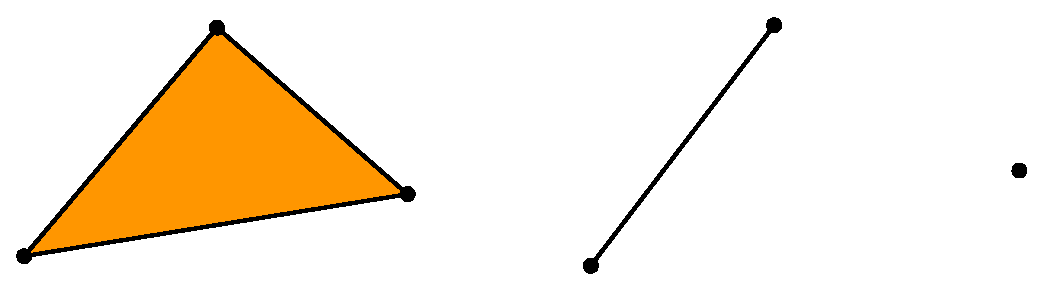
\includegraphics[width=0.9\textwidth]{bilder/inkscape/DreieckLiniePunkt.eps}
    \end{block}
  }

  \begin{frame}
    \begin{block}{Ein \textbf{Simplizialkomplex} \( K \) der \textbf{Dimension} \( n \) ist eine Menge von Simplizes \( \left\{\sigma^{p} \in \R^{N} \middle| 0 \le p \le n \le N \right\}\), so dass}
      \begin{enumerate}[(i)]
        \item \( \forall \sigma^{r} \prec \sigma^{p} :\quad \sigma^{r} \in K \qquad (0 \le r \le p) \)
        \item für alle \( \sigma^{r} := \sigma^{p} \cap \sigma^{q} \) gilt \( \qquad (0 \le r \le \min\{p,q\}) \)
              \begin{enumerate}[(a)]
                \item entweder \( \sigma^{r} \prec \sigma^{p}\) und  \( \sigma^{r} \prec \sigma^{q}\)
                \item oder \( \sigma^{r} = \emptyset \)
              \end{enumerate}
      \end{enumerate}
    \end{block}
    D.h. z.B. hängende Knoten sind nicht zulässig.
    \begin{block}{Das \textbf{Polytop} von \( K \) ist (der zu Grunde liegende Raum)}
      \[ |K| := \bigcup_{\sigma \in K} \sigma \]
    \end{block}
    (Andersherum heißt \( K \) eine \textbf{Triangulation} von \( |K| \))\\ 
    Achtung: \( |K| \) liegt nur für \textbf{flache} (\textbf{lineare}) \( K \) in einem affinen \( n \)-dim. Untervektoraum des \( \R^{N} \).
  \end{frame}

  \begin{frame}
    \begin{block}{Diskretisierung einer Mannigfaltigkeit \( M \)}
      \begin{itemize}
        \item Wir wollen nicht die Kartengebiete auf der Mannigfaltigkeit diskretisieren.
        \item Die \( n \)-Mannigfaltigkeit wird in den \( \R^{N} \) eingebettet.
        \item Wir setzen dann nur voraus, dass \( \sigma^{0}_{M} = \sigma^{0}_{K} \)
      \end{itemize}
    \end{block}
    \begin{block}{Beispiel}
      \centering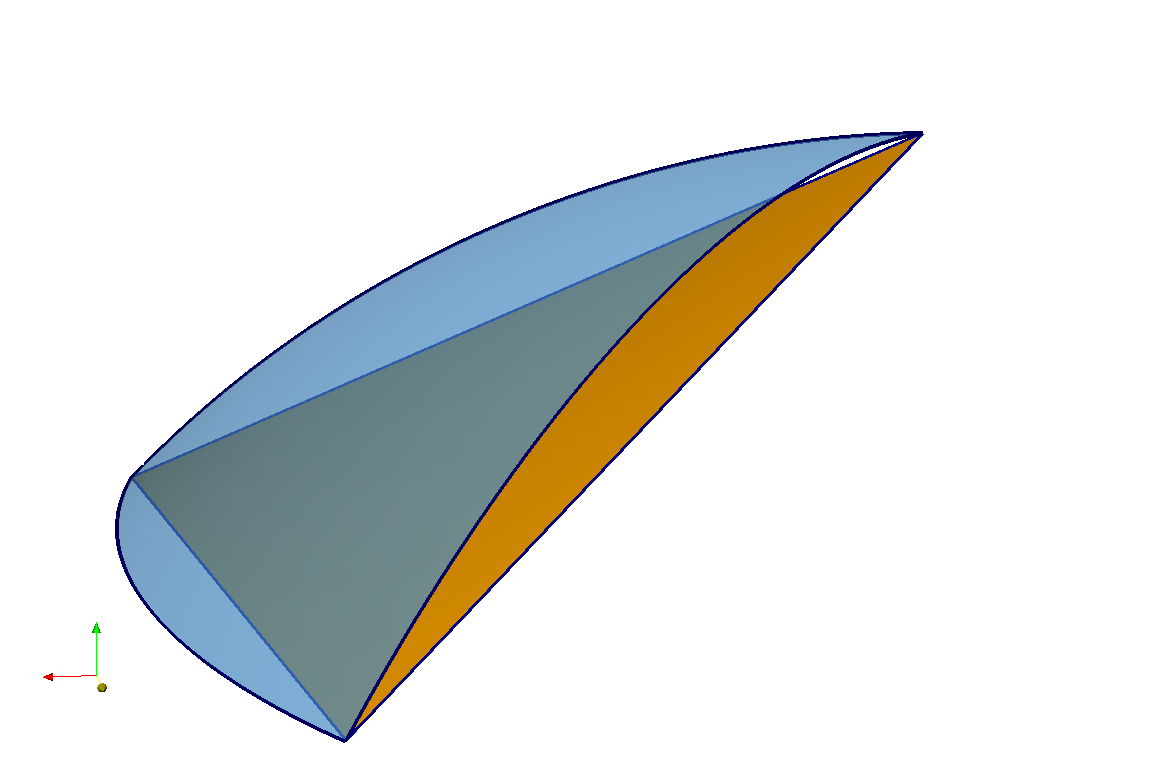
\includegraphics[width=0.5\textwidth]{bilder/paraview/abstractSimplex.png}
    \end{block}
  \end{frame}

  \begin{frame}
    \begin{block}{\textbf{Orientierter mannigfaltigartiger Simplizialkomplex} \( K \) (\textbf{Primärgitter})}
      \begin{description}
        \item[orientiert:] \( \sgn(\sigma^{n}_{1}, \sigma^{n}_{2}) = +1 \) für \( \sigma^{n}_{1} \cap \sigma^{n}_{2} \ne \emptyset \)
        \item[mannigfaltigartig:] \( |K| \) ist eine \( \mathfrak{C}^{0} \)-Mannigfaltigkeit
      \end{description}
    \end{block}
    \begin{block}{Beispiel}
      \centering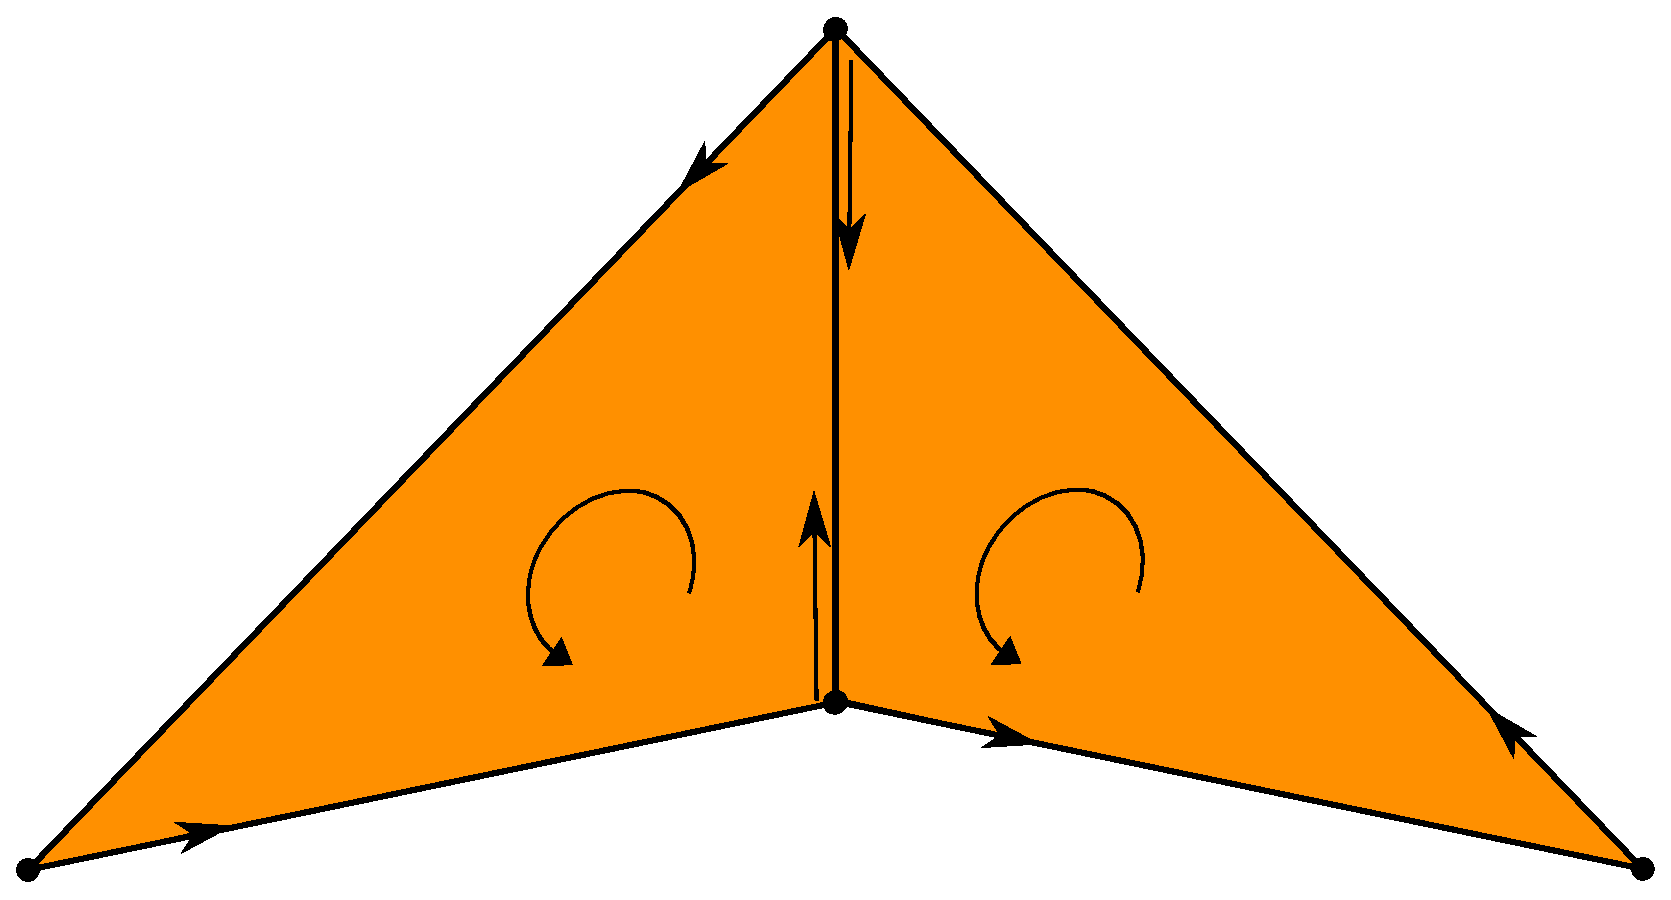
\includegraphics[width=0.6\textwidth]{bilder/inkscape/2Dreiecke.eps}
    \end{block}
    Durch lokale Nummerierung der Knoten (z.B. im math. pos. Drehsinn) auf den Volumenelementen \( \sigma^{n} \) lässt sich eine Orientierung induzieren.
  \end{frame}

  \begin{frame}
    \begin{block}{Umkreismittelpunkt (Circumcenter) \( c(\sigma^{p}) \)}
      \[ c(\sigma^{0}) := \sigma^{0} \]
      \[ v_{0},\ldots,v_{p} \in \mathds{S}^{p-1}_{c(\sigma^{p})} \subset P(\sigma^{p}) \]
    \end{block}
    \begin{block}{Wohlzentrierter Simplizialkomplex \( K \)}
    \[ \forall \sigma \in K :\quad c(\sigma) \in \text{Int}(\sigma) \]
    \end{block}

    \begin{minipage}{0.5\textwidth}
      (\( \text{Int}(\sigma^{0}) = \sigma^{0} \), \( \text{Bd}(\sigma^{0}) = \emptyset \))\\\\
      Die Wohlzentriertheit lässt sich durch Verfeinerung sicherstellen.
    \end{minipage} \, 
    \begin{minipage}{0.4\textwidth}
      \begin{block}{Beispiel}
        \centering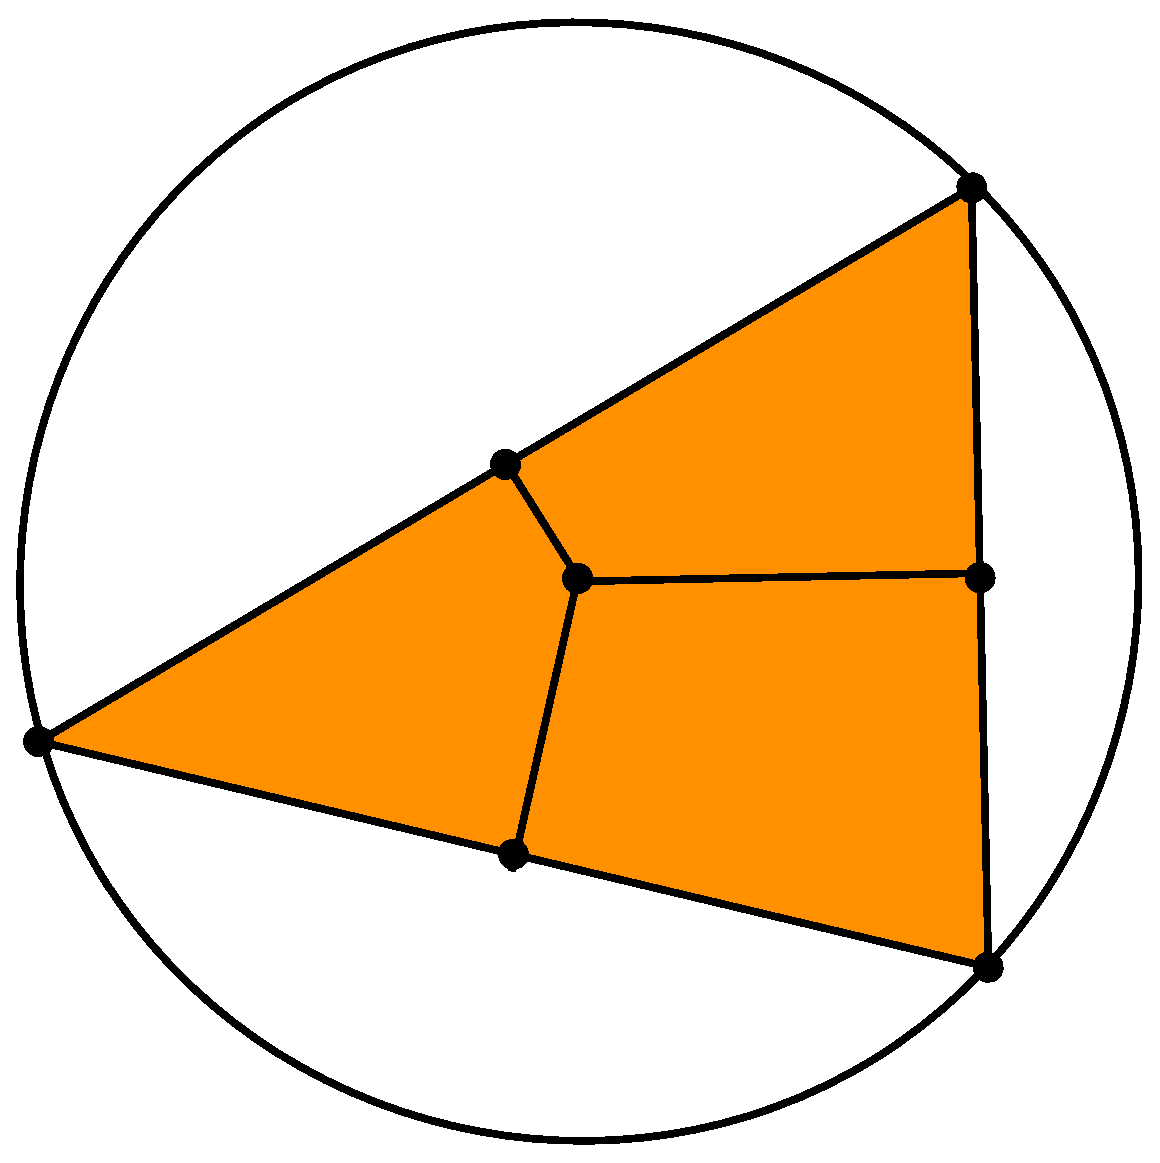
\includegraphics[width=0.6\textwidth]{bilder/inkscape/subdivision.eps}
      \end{block}
    \end{minipage}
  \end{frame}

  \begin{frame}
    \begin{block}{Umkreismittelpunktunterteilung eines wohlzentrierten Simplizialkomplexes (Circumcentric SubDivision)}
      \[ \text{csd}K := \left\{ \left[c(\sigma_{1}),\ldots,c(\sigma_{k})\right] \middle| \sigma_{1} \prec \ldots \prec \sigma_{k}, 1 \le k \le n \right\} \]
    \end{block}
    \begin{minipage}{0.5\textwidth}
      \begin{itemize}
        \item \( |\text{csd}K| = |K| \)
        \item Umsetzbar als Verfeinerung ohne Oberflächenprojektion
        \item Vorsicht: csd induziert eine andere Kantenorientierung als die oben angegebene.
        \item Ist \( K \) ein Primärgitter, dann ist \( \text{csd}K \) das Dualgitter.
      \end{itemize}
    \end{minipage} \, 
    \begin{minipage}{0.45\textwidth}
      \begin{block}{Beispiel}
        \centering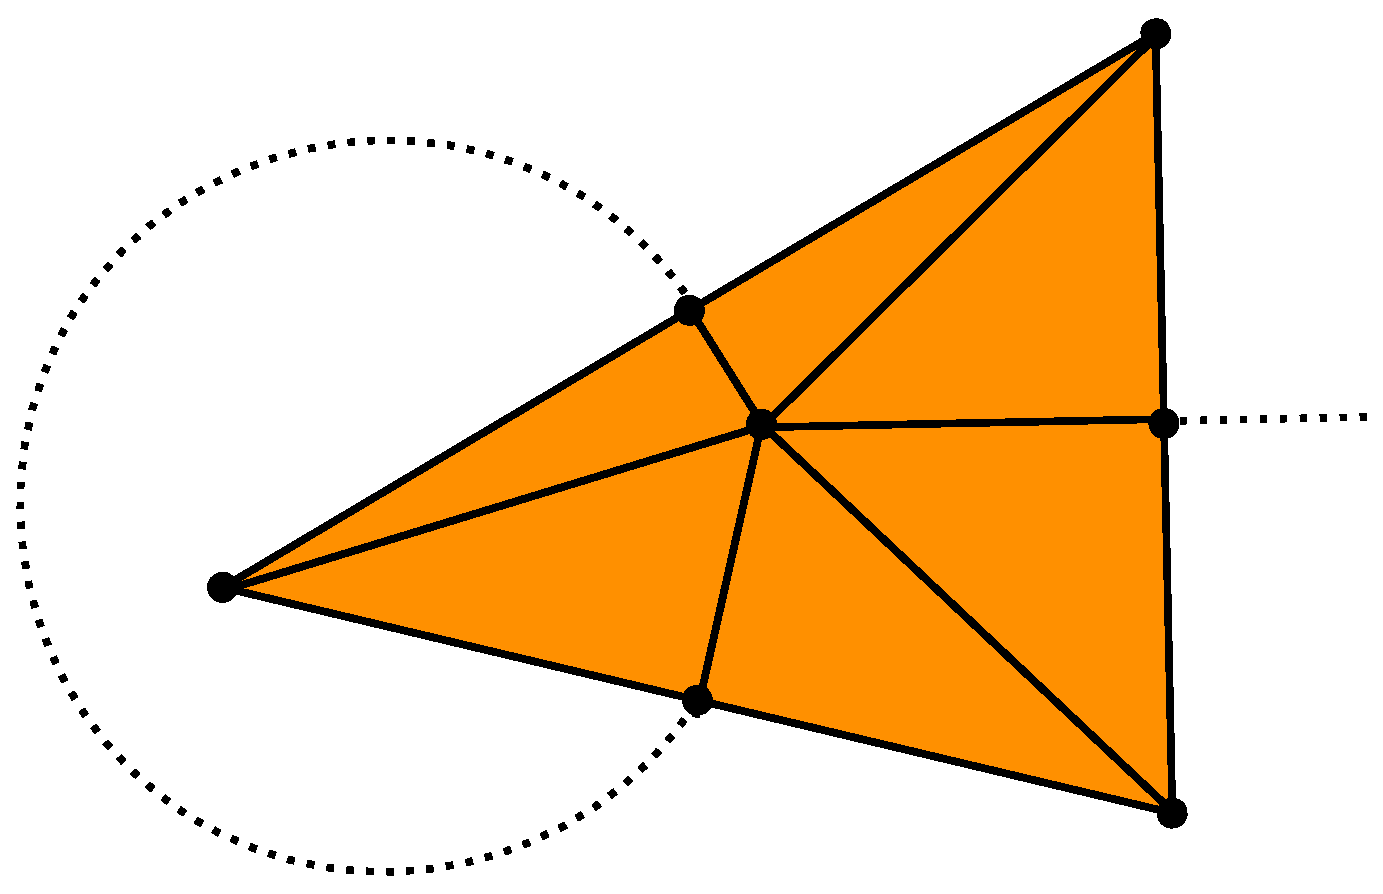
\includegraphics[width=0.99\textwidth]{bilder/inkscape/subdivision2.eps}
      \end{block}
    \end{minipage}
  \end{frame}

  
  \section{Differentialformen und diskrete Formen in 2D}

  \begin{frame}
    \begin{block}{Der Raum der \( p \)-Formen \( \Omega^{p}(M) \) auf einer (2-)Mannigfaltigkeit \( M \)}
      \( x \in M \):
      \begin{itemize}
        \item allg.: \(\Omega^{p}_{x}(M) = \mathfrak{A}(\left( T_{x}M \right)^{p}, \R) \subset \mathfrak{L}(\left( T_{x}M \right)^{p}, \R) \)
        \item \( \Omega^{0}_{x}(M) = \text{span}\left\{ 1 \right\} \), d.h. \( \Omega^{0}(M) = \mathfrak{C}^{\infty}(M, \R)\)
        \item \( \Omega^{1}_{x}(M) = \text{span}\left\{ dx^{1}, dx^{2} \right\} = T_{x}^{*}M = \mathfrak{L}(T_{x}M, \R) \) 
        \begin{itemize}
          \item \( dx^{i}\left(\frac{\partial}{\partial x^{j}}\right) = \delta_{i}^{j} \) (Dualität)
          \item \(\Omega^{p}(M) \overset{\flat\ \ \sharp}{\longleftrightarrow} \mathfrak{X}(M)\)
          \item  \( \alpha = \sum_{i}\alpha_{i}dx^{i} \in \Omega^{1}(M) \), \( v = \sum_{i}v^{i}\frac{\partial}{\partial x^{i}} \in \mathfrak{X}(M)  \):\\
              \( \qquad \alpha(v) = \sum_{i}\alpha_{i}v^{i} = \sum_{i,j}g_{ij}\alpha^{j}v^{i} = \langle \alpha^{\sharp}, v \rangle_{M} \)\\
              (Beziehung zum Skalarprodukt)
        \end{itemize}
        \item \( \Omega^{2}_{x}(M) = \text{span}\left\{ dx^{1} \wedge dx^{2}\right\} \subset \mathfrak{L}(T_{x}M \times T_{x}M, \R) \)
        \begin{itemize}
          \item \( \left(dx^{1}\wedge dx^{2}\right) \left(\frac{\partial}{\partial x^{1}}, \frac{\partial}{\partial x^{2}}\right)
              = -\left(dx^{1}\wedge dx^{2}\right) \left(\frac{\partial}{\partial x^{2}}, \frac{\partial}{\partial x^{1}}\right) = 1 \)
              (alternierend)
        \end{itemize}
      \end{itemize}
    \end{block}
  \end{frame}

  \begin{frame}
    \begin{block}{(Primärer) Kettenkomplex \( C_{p}(K) \)}
      \begin{itemize}
        \item \( C_{p}(K) = \text{span}\left\{ \sigma^{p} \in K \right\} \text{ (formal)}\)
        \item \( c^{p} \in C_{p}(K) \) heißt (primäre) p-Kette.
      \end{itemize}
    \end{block}
    \begin{block}{Beispiel}
      \centering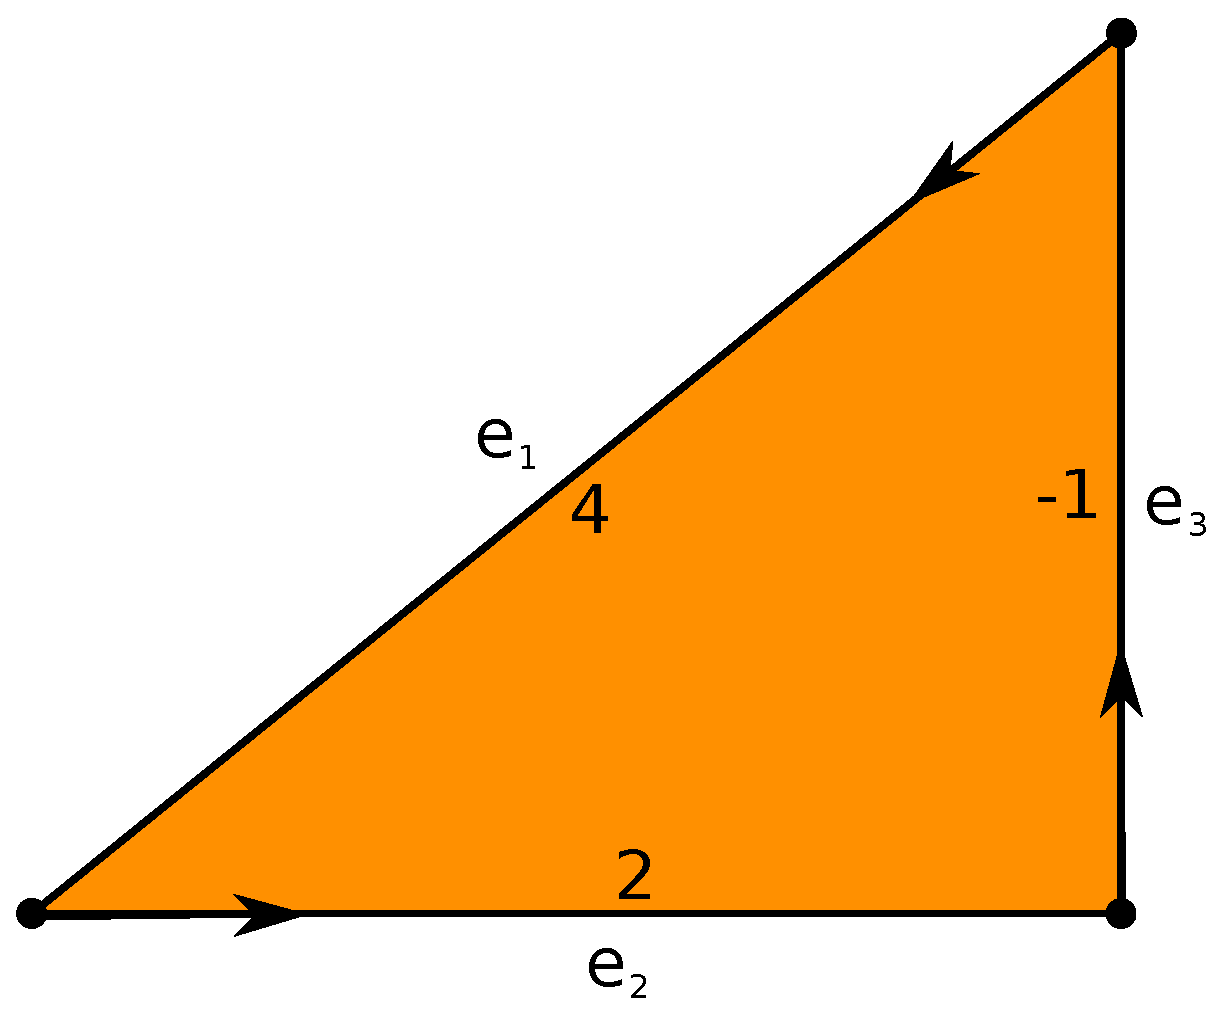
\includegraphics[width=0.4\textwidth]{bilder/inkscape/bspKette.eps}
      \[ c^{1} =  4e_{1} + 2e_{2} - e_{3} \in C_{1}(K) \]
    \end{block}
  \end{frame}

  \begin{frame}
    \begin{block}{Raum der (primären) diskreten \( p \)-Formen }
      \[ \Omega^{p}_{d}(K) := C^{p}(K) := \mathfrak{L}(C_{p}(K), \R) \]
    \end{block}
    \begin{block}{Von \( p \)-Formen zu diskreten \( p \)-Formen}
      \begin{itemize}
        \item Projektion eines Simplexes auf die Mannigfaltigkeit (abstraktes Simplex):
          \[ \pi: K \ni \sigma^{p} \longmapsto \pi(\sigma^{p}) =: \tau^{p} \in L \quad (\tau^{p} \subset M)  \]
        \item De-Rham-Abbildung \( \psi^{p}: \Omega^{p}(M) \rightarrow C^{p}(L)\):
          \[ \langle\psi^{p}(\alpha) , \tau^{p} \rangle := \psi^{p}(\alpha)(\tau^{p}) :=\int_{\tau^{p}} \alpha  \]
        \item diskrete \( p \)-Form \( \alpha_{d} \in C^{p}(K)\) einfach durch \( \psi(\alpha)\circ\pi \), d.h. 
          \[ \langle \alpha_{d} , \sigma^{p} \rangle := \alpha_{d}(\sigma^{p}) := \langle \psi^{p}(\alpha) , \pi(\sigma^{p}) \rangle\]
      \end{itemize}
    \end{block}
  \end{frame}
 
  \begin{frame}
    \begin{block}{Beispiel: diskrete 1-Form im Limes}
      \begin{align*}
        \alpha_{d}(\sigma_{\eps}^{1}) &= \langle \psi^{1}(\alpha) , s_{\eps} \rangle = \int_{s_{\eps}}\alpha = \int_{-\eps}^{\eps} \langle \alpha , \dot{s}_{\eps}(t) \rangle_{M} dt \\
                                 &= 2\eps \langle \alpha , v \rangle_{M} + \mathcal{O}(\eps^{3}\max_{\tau}\|\ddot{s}_{\eps}(\tau)\|) \text{ bei } x_{0} \\
        \Rightarrow\quad  & \frac{1}{|\sigma^{1}_{\eps}|} \alpha_{d}(\sigma_{\eps}^{1}) = \alpha_{d}(v) = \alpha(v) +  \mathcal{O}(\eps^{2}\max_{\tau}\|\ddot{s}_{\eps}(\tau)\|)
      \end{align*}
      \centering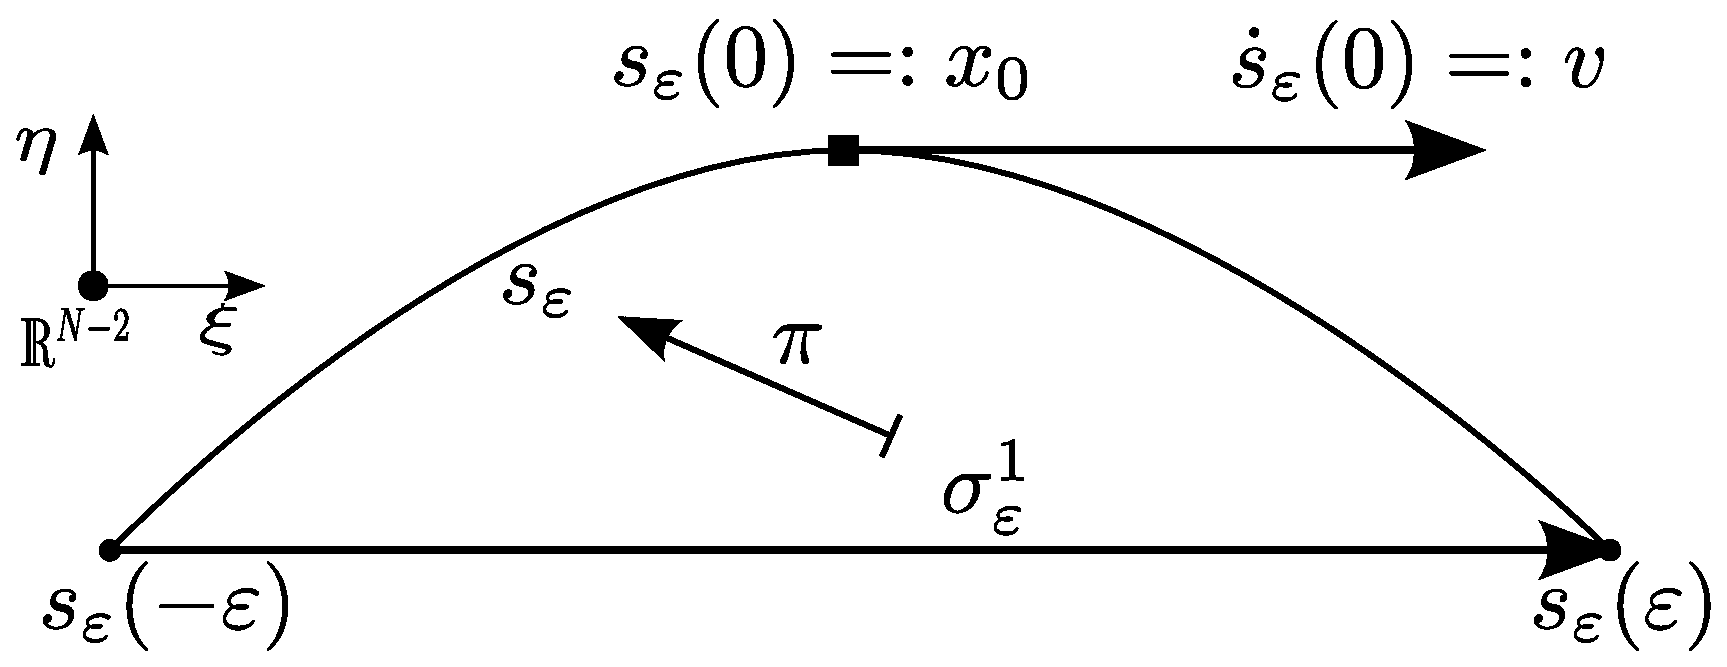
\includegraphics[width=0.8\textwidth]{bilder/inkscape/EpsilonKette.eps}\\
      (\( s_{\eps} \) so parametrisiert, dass \( \|v\|_{\R^{N}} = 1 \))
    \end{block}
  \end{frame}

  

  \section{Äußere Ableitung}

  \begin{frame}
    \begin{block}{Äußere (Cartan) Ableitung \( \d: \Omega^{p}(M) \longrightarrow \Omega^{p+1}(M) \) auf einer (2-)Mannigfaltigkeit \( M \)}
      \begin{itemize}
        \item \( f \in \Omega^{0}(M):\quad \d f = \ablx{f}{1}dx^{1} + \ablx{f}{2}dx^{2} \in  \Omega^{1}(M)\)
        \item \( \alpha = \alpha_{1}dx^{1} + \alpha_{2}dx^{2} \in \Omega^{1}(M):\) 
                \[\d\alpha = \left( \ablx{\alpha_{2}}{1} - \ablx{\alpha_{1}}{2} \right) dx^{1} \wedge dx^{2} \in \Omega^{2}(M)\]
        \item \( 0 \rightarrow \mathfrak{C}^{\infty}(M) \overset{\d_{0}}{\rightarrow} \Omega^{1}(M) \overset{\d_{1}}{\rightarrow} \Omega^{2}(M) \rightarrow 0\) \\
              (\( \nearrow \) De-Rham-Kohomologie)
        \item d.h. \( \d\circ\d = 0 \)
        \item Stokes' Theorem: 
            \[ \int_{M}\d\omega = \int_{\partial M} \omega \qquad (\omega\in\Omega^{p}(M))\]
            (Kurzschreibweise, eigentlich \( \int_{\partial M} i^{*}\omega \) auf der RHS mit \( i: \partial M \rightarrow M \))
      \end{itemize}
    \end{block}
  \end{frame}

  \begin{frame}
    \begin{block}{Randoperator \( \partial:C_{p}(K) \longrightarrow C_{p-1}(K) \)}
      \[ \partial\sigma^{p} = \partial\left[ v_{0}, \ldots, v_{p} \right] = \sum_{i=0}^{p} (-1)^{p} \left[ v_{0}, \ldots, \hat{v}_{i}, \ldots,  v_{p} \right]\]
      \begin{itemize}
        \item \( \partial\left[ v_{0}, v_{1}, v_{2} \right] = \left[ v_{1}, v_{2} \right] - \left[ v_{0}, v_{1} \right] + \left[ v_{0}, v_{1} \right]\)
        \item \( \partial\left[ v_{0}, v_{1} \right] = \left[ v_{0} \right] - \left[ v_{1} \right]\)
        \item \( \partial\circ\partial = 0 \) \qquad(\( \nearrow \) Kettenkomplex)
      \end{itemize}
    \end{block}
  \end{frame}

  \begin{frame}
    \begin{block}{Diskrete Äußere Ableitung (Korandoperator) \( \d: \Omega_{d}^{p}(K) \longrightarrow \Omega_{d}^{p+1}(K) \)}
      \[ \d\alpha := \alpha\circ\partial \]
      \begin{itemize}
        \item d.h. \( \left\langle \d\alpha , c_{p+1} \right\rangle =  \left\langle \alpha , \partial c_{p+1} \right\rangle\) 
              \qquad(Diskretes Stokes' Theorem)
        \item \( \d\circ\d = 0 \) \qquad(\( \nearrow \) Kokettenkomplex)
      \end{itemize}
    \end{block}
    \begin{block}{Beispiel: Rücktransport (Pullback) einer diskreten Form \( \alpha\in\Omega_{d}^{p}(K)\) bzgl. \( \varphi:|\tilde{K}|\rightarrow |K| \)}
      \begin{align*}
        \left\langle \varphi^{*}(\d \alpha) , \sigma^{p+1} \right\rangle &= \left\langle \d \alpha , \varphi\sigma^{p+1} \right\rangle
                                                                          = \left\langle \alpha , \partial(\varphi\sigma^{p+1}) \right\rangle
                                                                          =  \left\langle \varphi^{*}\alpha , \partial\sigma^{p+1} \right\rangle \\
                                                                         &= \left\langle \d(\varphi^{*}\alpha) , \sigma^{p+1} \right\rangle
      \end{align*}
    \end{block}
    (\( \varphi^{*}\alpha \in \Omega_{d}^{p}(\tilde{K}) \) ist dann die zurückgezogene diskrete Form)
  \end{frame}




  \section{Hodge-Operator}

  \begin{frame}
    \begin{block}{Hodge-Stern-Operator \( *: \Omega^{p}(M) \longrightarrow \Omega^{n-p}(M)\) auf einer (2-)Mannigfaltigkeit \( M \) (mit Metrik \( g = \text{diag}(g_{1}, g_{2}) \))}
      \begin{itemize}
        \item \( * \circ * = (-1)^{p(n-p)}\text{Id} \) \qquad (für \( \text{Ind}(M) = 0 \))
        \item \( f \in \Omega^{0}(M):\quad * f = f \sqrt{|g|} dx^{1}\wedge dx^{2}  = f\mu\) 
        \item \( \alpha = \alpha_{1}dx^{1} + \alpha_{2}dx^{2} \in \Omega^{1}(M):\) 
              \[ *\alpha = \sqrt{|g|} \left( g^{1} \alpha_{1}dx^{2} - g^{2} \alpha_{2}dx^{1} \right) = \sqrt{|g|} \left( \alpha^{1}dx^{2} - \alpha^{2}dx^{1} \right)\]
        \item \( \omega = \omega_{12}dx^{1}\wedge dx^{2} \in \Omega^{2}(M):\qquad *\omega = \frac{1}{\sqrt{|g|}}\omega_{12} \)
        \item Allgemeine Definition: \( \alpha \wedge *\beta = \left\langle \alpha , \beta \right\rangle \mu\) für \( \alpha, \beta \in \Omega^{p}(M) \)\\
              \( \Rightarrow *\left( dx^{i_{1}} \wedge \ldots \wedge dx^{i_{p}} \right) 
                  = \sqrt{|g|} \sum_{\begin{smallmatrix}
                                          j_{1}<\ldots<j_{p} \\
                                          j_{p+1}<\ldots<j_{n}
                                     \end{smallmatrix}} \text{sgn}\left( j_{1}, \ldots, j_{n} \right) g^{i_{1}j_{1}}\ldots g^{i_{p}j_{p}} dx^{j_{p+1}} \wedge \ldots \wedge dx^{j_{n}}\)
      \end{itemize}
    \end{block}
  \end{frame}

  \begin{frame}
    \begin{block}{(Stern-)Dualitätsoperator \( \star: C_{p}(K) \longrightarrow C_{n-p}(\text{csd}K) \)}
      \[ \star(\sigma^{p}) = \sum_{\sigma^{p} \prec \ldots \prec \sigma^{n}} s_{\sigma^{p},\ldots,\sigma^{n}} \left[ c(\sigma^{p}),\ldots,c(\sigma^{n}) \right]  \]
      wobei für beliebige \( \sigma^{0} \prec \ldots \prec \sigma^{p-1} \prec \sigma^{p} \) aus \( K \):
      \[ s_{\sigma^{p},\ldots,\sigma^{n}} = \text{sgn}\left( \left[ c(\sigma^{0}),\ldots,c(\sigma^{p}) \right], \sigma^{p} \right) 
                                      \cdot \text{sgn}\left( \left[ c(\sigma^{0}),\ldots,c(\sigma^{n}) \right], \sigma^{n} \right) \]
    \end{block}
    \begin{block}{Beispiel: 2D}
      \begin{itemize}
        \item Knoten (\( \sigma^{0} \)) werden auf die  Voronoi-\glqq Zellen\grqq (-Flächenketten) abgebildet.
          (Orientierungen sind gleich der anderen Flächensimplexe \(\Leftarrow\) Orientierbarkeit) 
        \item Kanten (\( \sigma^{1} \)) werden auf die Voronoi-\glqq Kanten\grqq (-Kantenketten) abgebildet.
          (Orientierung (bei Rechte-Hand-Ambiente) durch Vierteldrehung von \( \sigma^{1} \) gegen den Uhrzeigersinn)
        \item Flächen (\( \sigma^{2} \)) werden auf die Voronoi-Knoten abgebildet. (Orientierung ist \( +1 \) per Def.)
      \end{itemize}
    \end{block}
  \end{frame}
    
  \begin{frame}
    \begin{block}{Beispiel: 2D}
      \centering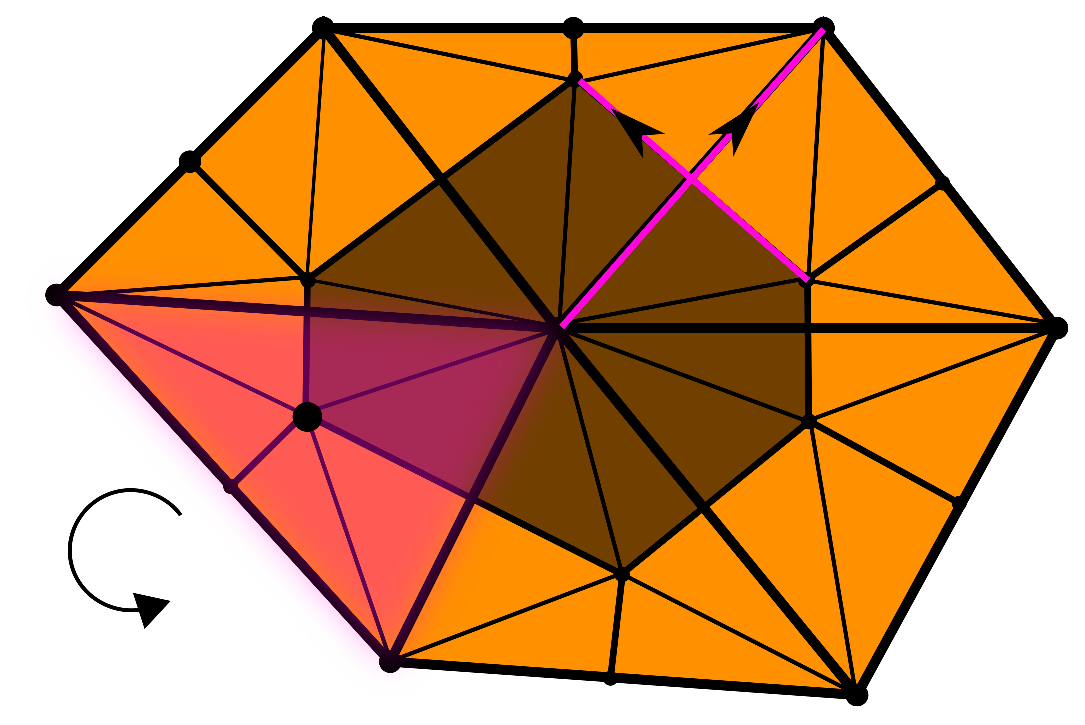
\includegraphics[width=0.9\textwidth]{bilder/inkscape/dualSigma0.eps}
    \end{block}
  \end{frame}

  \begin{frame}
    \begin{block}{Dualer Kettenkomplex (Voronoikomplex) \( C_{p}(\star K) \)}
      \[ C_{p}(\star K) := \text{Im}(\star_{n-p}) \le C_{p}(\text{csd}K) \]
    \end{block}
    \begin{block}{(Stern-)Dualitätsoperator \( \star: C_{p}(\star K) \longrightarrow C_{n-p}(K)\), so dass gilt}
      \[ \star\star \sigma^{n-p} = (-1)^{p(n-p)}\sigma^{n-p}\]
    \end{block}
    \begin{block}{Beispiel: Kante \( \sigma^{1} \) in 2D}
      \glqq Two Quarter Turns Make a Flip \grqq
    \end{block}
    \begin{block}{Raum der dualen diskreten \( p \)-Formen }
      \[ \Omega^{p}_{d}(\star K) := C^{p}(\star K) := \mathfrak{L}(C_{p}(\star K), \R) \]
    \end{block}
  \end{frame}

  \begin{frame}
    \begin{block}{Diskreter Hodge-Stern-Operator \( *: \Omega^{p}(K) \longrightarrow \Omega^{n-p}(\star K)\)}
      \[ \frac{1}{|\star\sigma^{p}|} \left\langle *\alpha , \star\sigma^{p} \right\rangle := \frac{s}{|\sigma^{p}|} \left\langle \alpha , \sigma^{p} \right\rangle\]
      \begin{itemize}
        \item Für \( 1 \le p \le n-1: \qqquad s = 1 \)
        \item Für \( p = 0: \qqquad s = (-1)^{n-1} \text{sgn} \left( \partial(\star\sigma^{0}), \star\sigma^{1} \right) \)
              \begin{itemize}
                \item Kante \( \sigma^{1} \succ \sigma^{0} \) zeigt von \( \sigma^{0} \) weg.
                \item In 2D (bei Rechte-Hand-Ambiente) ist \( s = -1 \).
              \end{itemize}
              \item Für \( p = n:\)      
     \[s = \begin{cases} (-1)^{n-1} & \text{ falls für } \tilde{\sigma}^{n-1} \subset \partial \sigma^{n} \text { die } \star\tilde{\sigma}^{n-1} \text{ von } \star\sigma^{n} \text{ wegzeigen,} \\
                         (-1)^{n} & \text{ sonst.}
           \end{cases}\]
                \begin{itemize}
                  \item In 2D ist \( s = 1 \).
                \end{itemize}
      \end{itemize}
    \end{block}
  \end{frame}

  
  
  \section{Koableitung}

  \begin{frame}
    \begin{block}{Koableitung \( \delta: \Omega^{p+1}(M) \longrightarrow \Omega^{p}(M) \) \qquad (Ind\( (M)=0 \))}
      \[ \delta := (-1)^{np+1} * \d * \]
      \begin{itemize}
        \item \( \delta\circ\delta = 0 \)
        \item \( \left\langle\left\langle \delta\alpha , \beta \right\rangle\right\rangle = \left\langle\left\langle \alpha , \d\beta \right\rangle\right\rangle \)
        \item Laplace-De-Rham: \( \Delta^{dR} := \delta\d + \d\delta \)
        \item Laplace-Beltrami: \( \Delta^{B} := \text{Div}\circ\text{Grad} := -\delta\d \)
        \item in 2D:
              \begin{itemize}
                \item \( \delta = - * \d * \)
                \item Laplace-Beltrami für eine \( 0 \)-Form \( f \) mit Metrik \( g=\text{diag}(g_{1}, g_{2}) \):
                      \[ \Delta^{B}f = \frac{1}{\sqrt{|g|}} \left[ \ablx{}{1}\left( \sqrt{|g|}g^{1}\ablx{f}{1}\right) +  \ablx{}{2}\left( \sqrt{|g|}g^{2}\ablx{f}{2}\right)\right] \]
              \end{itemize}
      \end{itemize}
    \end{block}
    (\( \alpha,\beta \in \Omega^{p}(M): \qquad \left\langle\left\langle \alpha , \beta \right\rangle\right\rangle = \int_{M}\alpha\wedge *\beta\))
  \end{frame}

\end{document}
